\documentclass[12pt]{article}
\usepackage[utf8]{inputenc}
\usepackage{amsmath}
\usepackage{amsfonts}
\usepackage{amssymb}
\usepackage{empheq}
\usepackage{graphicx}
\usepackage{tikz}
\usetikzlibrary{automata, positioning, arrows, shapes}
\addtolength{\topmargin}{-0.875in}
\addtolength{\textheight}{1.75in}

\title{Math 332 A - Mathematical Statistics}
\author{Ethan Jensen}
\date{January 31, 2020}

\begin{document}
	\maketitle HW p.250 \#38,40 \ p.257 \#80,81,82*,83*
	\section[20pt]{p. 250 \#38}
	Show that for \(\nu_2>2\) the mean of the \(F\) distribution is \(\frac{\nu_2}{\nu_2-2}\), making use of the definition of \(F\) in Theorem 8.14 and the fact that for a random variable V having the chi-square distribution with \(\nu_2\) degrees of freedom, \newline
	\(E\left(\frac{1}{V}\right)=\frac{1}{\nu_2-2}\).
	\newline \newline
	Let U and V be independent chi-square distributions with respective \(\nu_1\) and \(\nu_2\) degrees of freedom. \newline \newline
	With Theorem 8.14 we can write
	\[F = \frac{V/\nu_1}{U/\nu_2} \implies E(F) = E\left(\frac{V/\nu_1}{U/\nu_2}\right)\]
	Using Corollary 4.1, we can drag out the constants \(\nu_1\) and \(\nu_2\). \newline
	\[E(F) = \frac{\nu_2}{\nu_1}E\left(\frac{U}{V}\right)\]
	In class, we determined that if U and V are independent, then certainly U and \(\frac{1}{V}\) are independent. \newline
	Thus, by Thm. 4.12 we can write
	\[E(F) = \frac{\nu_2}{\nu_1}E(U)E\left(\frac{1}{V}\right)\]
	Since U is chi-square, we know that \(E(U)=\nu_1\) by Corollary 6.1. \newline
	From the problem, we miraculously know that
	\[E\left(\frac{1}{V}\right)=\frac{1}{\nu_2-2}\]
	Combining everything together and simplifying we have
	\[\mu_F = E(F)=\frac{\nu_2}{\nu_1}\frac{\nu_1}{\nu_2-2}=\frac{\nu_2}{\nu_2-2}\]
	\boxed{\textup{For } \nu_2 > 2, \textup{the mean of the F distribution is }\frac{\nu_2}{\nu_2-2}}
	\newline
	\maketitle HW p.250 \#38,40 \ p.257 \#80,81,82*,83*
	\section[20pt]{p. 250 \#40}
	Verify that if \(T\) has a t distribution with \(\nu\) degrees of freedom, the \(X=T^2\) has an F distribution with \(\nu_1 = 1\) and \(\nu_2=\nu\) degrees of freedom. \newline \newline
	Let Z and Y be independent random variables with respective standard normal and chi-square distribution with \(\nu\) degrees of freedom.
	By Theorem 8.12, \(X\) can be written as
	\[X=T^2=\left(\frac{Z}{\sqrt{Y/\nu}}\right)^2=\frac{Z^2}{Y/\nu}\]
	By Theorem 8.7, \(Z^2\) has the chi-square distribution with 1 degree of freedom. \newline
	Thus, X is a proportion of chi-square distributions, and thus has the F distribution by Theorem 8.14. \newline
	\(X=\frac{Z^2/1}{Y/\nu}\) \newline
	\boxed{\textup{X has the F distribution with }\nu_1 = 1 \textup{ and } \nu_2=\nu \textup{ degrees of freedom.}}
	\newline \newpage
	\maketitle HW p.250 \#38,40 \ p.257 \#80,81,82*,83*
	\section[20pt]{p. 257 \#80}
	A random sample of size \(n=25\) from a normal population has the mean \(\overline{x}=47\) and the standard deviation \(s=7\). If we base our decision on the statistic of Theorem 8.13, can we say that the given information supports the conjecture that the mean of the population is \(\mu=42\)? \newline \newline
	Theorem 8.13 states that \(T=\frac{\overline{X}-\mu}{S/\sqrt{n}}\) has the t-distribution with \(n-1\) degrees of freedom. \newline
	Plugging in our values for \(n,\overline{x},s,\) and \(\mu\) we have
	\(t=\frac{47-42}{7/5}=7\). \newline
	\newline
	Referring to Table IV, with \(\nu = 24\), getting a value greater than 3 for t is already extremely unlikely. \newline
	\boxed{\textup{The given information does not support the conjecture.}}
	\newline \newpage
	\maketitle HW p.250 \#38,40 \ p.257 \#80,81,82*,83*
	\section[20pt]{p. 257 \#81}
	A random sample of size \(n=12\) from a normal population has the mean \(\overline{x}=27.8\) and the variance \(s^2=3.24\). If we base our decision on the statistic of Theorem 8.13, can we say that the given information supports the claim that the mean of the population \(\mu = 28.5\)? \newline \newline
	Theorem 8.13 states that \(T=\frac{\overline{X}-\mu}{S/\sqrt{n}}\) has the t-distribution with \(n-1\) degrees of freedom. \newline
	Plugging in our values for \(n,\overline{x},s,\) and \(\mu\) we have
	\(t=\frac{27.8-28.5}{1.8/\sqrt{12}}\approx -1.34715\). \newline
	\newline
	Referring to Table IV with \(\nu = 11\), getting a value less than -1.34715 for t is 0.10. That's not that bad. \newline
	\boxed{\textup{The given information supports the conjecture.}}
	\newline \newpage
	\maketitle HW p.250 \#38,40 \ p.257 \#80,81,82*,83*
	\section[20pt]{p. 257 \#82}
	If \(S_1\) and \(S_2\) are the standard deviations of independent random samples of size \(n_1=61\) and \(n_2=31\) from normal populations with \(\sigma_1^2=12\) and \(\sigma_2^2=18\), find \(P(S_1^2/S_2^2>1.25)\). \newline \newline
	By Theorem 8.15 we can say that
	\[F=\frac{S_1^2\sigma_2^2}{S_2^2\sigma_1^2}\]
	is a random variable having an F distribution with \(n_1-1\) and \(n_2-1\) degrees of freedom. \newline
	Notice that
	\[P(S_1^2/S_2^2>1.25) = P(\frac{S_1^2\sigma_2^2}{S_2^2\sigma_1^2}>1.25\frac{\sigma_2^2}{\sigma_1^2})=P(f > 1.875)\]
	where f has an F distirbution with \(\nu_1=30\) and \(\nu_2=60\).
	Using Wolfram Alpha (not Excel), we calculate \(P(f > 1.875)\).
	\newline \newline
	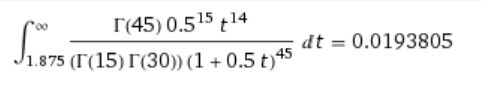
\includegraphics{spicy integral}
	\newline
	\boxed{P(f > 1.875) \approx 0.0193805}
	\newline \newpage
	\maketitle HW p.250 \#38,40 \ p.257 \#80,81,82*,83*
	\section[20pt]{p. 257 \#83}
	If \(S_1\) and \(S_2\) are the standard deviations of independent random samples of size \(n_1=10\) and \(n_2=15\) from normal populations with equal variances, find \(P(S_1^2/S_2^2<3.05)\). \newline \newline
	By Theorem 8.15 we can say that
	\[F=\frac{S_1^2\sigma_2^2}{S_2^2\sigma_1^2}\]
	is a random variable having an F distribution with \(n_1-1\) and \(n_2-1\) degrees of freedom. \newline
	Notice that
	\[P(S_1^2/S_2^2<3.05) = P(\frac{S_1^2\sigma_2^2}{S_2^2\sigma_1^2}>1.25\frac{\sigma_2^2}{\sigma_1^2})=P(f <3.05)\]
	where f has an F distirbution with \(\nu_1=9\) and \(\nu_2=14\).
	Using Wolfram Alpha (not Excel), we calculate \(P(f > 3.05)\).
	\newline \newline
	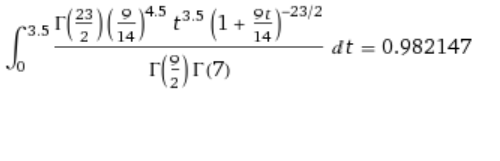
\includegraphics{spicy integral 2}
	\newline
	\boxed{P(f > 1.875) \approx 0.982147}

\end{document}
